%%
%% This is a template file for Tex
%%
%%It provides framework for UML(including Flow Chart)
%%
%%
%%
%%

\documentclass[11pt,a4paper]{article}
\usepackage{fontspec}
\usepackage{tikz}
\usepackage{tikz-uml}

%%\setmainfont[BoldFont=Adobe Heiti Std]{Adobe Song Std}
\setmainfont{SimSun}
%%\setsansfont[BoldFont=Adobe Heiti Std]{AR PL KaitiM GB}
%%\setmonofont{Bitstream Vera Sans Mono}
\begin{document}
世界,你好!

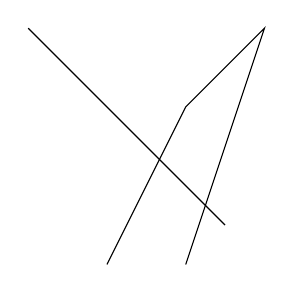
\begin{tikzpicture}
\draw (0,0) --(1,2) -- (2,3) -- (1,0);
\draw (-1,3) --(1.5, 0.5);
\end{tikzpicture}


\begin{tikzpicture} \draw [yellow, line width=6] (0,0) -- (.5,0); \end{tikzpicture} you want

\begin{tikzpicture}

\umlclass[x=0, y=-3] {namespace::class1\_name}{}{}
\umlclass[x=0, y=-7, width=35ex] {namespace::class2\_name}{}{}
\umlclass[x=8, y=-5] {namespace::class3\_name}{}{}
\umlclass[x=0, y=-10] {namespace::class4\_name} {}{}
\umluniaggreg [arg1=*, mult1=1, arg2=a, mult2=1] {namespace::class1\_name} {namespace::class2\_name}
\umluniaggreg [arg2=b, mult2=1,pos=0.95] {namespace::class1\_name} {namespace::class3\_name}
\umlinherit {namespace::class4\_name}{namespace::class3\_name}
\umlinherit {namespace::class4\_name}{namespace::class2\_name}

\begin{umlpackage} [x=0, y=0] {My First Package 包1}
\end{umlpackage}

\begin{umlpackage} [x=7, y=-3] {My Second Package 包2}
\end{umlpackage}
%%\end{tikzpicture}

\begin{umlsystem} [x=5,y=5] {use case system}
%%\umlactor [scale=0.5] {small user}
\umlusecase [name=c2] {Case 2}
\umlusecase [x=1, y=-2, name=c3] {Case 3}
\umlusecase [y=-4, name=c5] {Case 5}
\umlinclude {c2} {c3}
\umlinherit {c5} {c3}
\end{umlsystem}
\umlactor [x=0, y=5, scale=0.7] {user}
\umlassoc {user}{c2}
\umlassoc {user} {c5}
\umlusecase [x=5, y=5, name=c1] { case 1}
%%\begin{tikzpicture}
\end{tikzpicture}

\end{document}
